\documentclass[11pt,a4paper]{article}
% Shared preamble for the NAIL094 reports
% Used by every task via % Shared preamble for the NAIL094 reports
% Used by every task via % Shared preamble for the NAIL094 reports
% Used by every task via \input{../../shared/preamble}

\usepackage[T1]{fontenc}
\usepackage[utf8]{inputenc}
\usepackage{lmodern}
\usepackage[margin=2.5cm]{geometry}

\usepackage{amsmath}
\usepackage{amssymb}
\usepackage{booktabs}
\usepackage{float}
\usepackage{graphicx}
\usepackage{listings}
\usepackage{xcolor}
\usepackage{caption}

\usepackage[hidelinks]{hyperref}

\setlength{\parskip}{0.5em}
\setlength{\parindent}{0pt}

% Title fields, set these in the report before \begin{document}
\makeatletter
\newcommand{\reportcourse}[1]{\def\@reportcourse{#1}}
\newcommand{\reporttask}[1]{\def\@reporttask{#1}}
\newcommand{\reportauthor}[1]{\def\@reportauthor{#1}}

\newcommand{\makereporttitle}{%
  \begin{center}
    {\LARGE\bfseries \@reportcourse \par}
    \vspace{0.8em}
    {\Large \@reporttask \par}
    \vspace{0.6em}
    {\normalsize \@reportauthor \par}
  \end{center}
  \vspace{1em}
  \hrule
  \vspace{1.5em}
}
\makeatother

% Inline code
\newcommand{\code}[1]{\texttt{#1}}

% Code listings
\lstdefinestyle{reportcode}{
  basicstyle=\ttfamily\small,
  keywordstyle=\color{blue!60!black},
  commentstyle=\color{gray},
  stringstyle=\color{green!40!black},
  breaklines=true,
  showstringspaces=false,
  frame=single,
  rulecolor=\color{gray!40},
  numbers=none,
}
\lstset{style=reportcode}


\usepackage[T1]{fontenc}
\usepackage[utf8]{inputenc}
\usepackage{lmodern}
\usepackage[margin=2.5cm]{geometry}

\usepackage{amsmath}
\usepackage{amssymb}
\usepackage{booktabs}
\usepackage{float}
\usepackage{graphicx}
\usepackage{listings}
\usepackage{xcolor}
\usepackage{caption}

\usepackage[hidelinks]{hyperref}

\setlength{\parskip}{0.5em}
\setlength{\parindent}{0pt}

% Title fields, set these in the report before \begin{document}
\makeatletter
\newcommand{\reportcourse}[1]{\def\@reportcourse{#1}}
\newcommand{\reporttask}[1]{\def\@reporttask{#1}}
\newcommand{\reportauthor}[1]{\def\@reportauthor{#1}}

\newcommand{\makereporttitle}{%
  \begin{center}
    {\LARGE\bfseries \@reportcourse \par}
    \vspace{0.8em}
    {\Large \@reporttask \par}
    \vspace{0.6em}
    {\normalsize \@reportauthor \par}
  \end{center}
  \vspace{1em}
  \hrule
  \vspace{1.5em}
}
\makeatother

% Inline code
\newcommand{\code}[1]{\texttt{#1}}

% Code listings
\lstdefinestyle{reportcode}{
  basicstyle=\ttfamily\small,
  keywordstyle=\color{blue!60!black},
  commentstyle=\color{gray},
  stringstyle=\color{green!40!black},
  breaklines=true,
  showstringspaces=false,
  frame=single,
  rulecolor=\color{gray!40},
  numbers=none,
}
\lstset{style=reportcode}


\usepackage[T1]{fontenc}
\usepackage[utf8]{inputenc}
\usepackage{lmodern}
\usepackage[margin=2.5cm]{geometry}

\usepackage{amsmath}
\usepackage{amssymb}
\usepackage{booktabs}
\usepackage{float}
\usepackage{graphicx}
\usepackage{listings}
\usepackage{xcolor}
\usepackage{caption}

\usepackage[hidelinks]{hyperref}

\setlength{\parskip}{0.5em}
\setlength{\parindent}{0pt}

% Title fields, set these in the report before \begin{document}
\makeatletter
\newcommand{\reportcourse}[1]{\def\@reportcourse{#1}}
\newcommand{\reporttask}[1]{\def\@reporttask{#1}}
\newcommand{\reportauthor}[1]{\def\@reportauthor{#1}}

\newcommand{\makereporttitle}{%
  \begin{center}
    {\LARGE\bfseries \@reportcourse \par}
    \vspace{0.8em}
    {\Large \@reporttask \par}
    \vspace{0.6em}
    {\normalsize \@reportauthor \par}
  \end{center}
  \vspace{1em}
  \hrule
  \vspace{1.5em}
}
\makeatother

% Inline code
\newcommand{\code}[1]{\texttt{#1}}

% Code listings
\lstdefinestyle{reportcode}{
  basicstyle=\ttfamily\small,
  keywordstyle=\color{blue!60!black},
  commentstyle=\color{gray},
  stringstyle=\color{green!40!black},
  breaklines=true,
  showstringspaces=false,
  frame=single,
  rulecolor=\color{gray!40},
  numbers=none,
}
\lstset{style=reportcode}


\reportcourse{NAIL094 --- Decision Procedures and SAT/SMT Solvers}
\reporttask{Testing Equivalence}
\reportauthor{Zerina Ahmetovic}

\begin{document}
\makereporttitle

\section{Task overview}

The task is to write a program that decides the logical relationship between
two CNF formulas. As input the program is given two files in DIMACS format,
the same format as in the first task, representing the formulas $\varphi$ and
$\psi$. On the output the program prints whether
$\varphi \Leftrightarrow \psi$, $\varphi \Rightarrow \psi$,
$\varphi \Leftarrow \psi$, or none of these holds.

The implication $\varphi \Rightarrow \psi$ holds for every assignment if its negation
is unsatisfiable, which reduces to checking that $\varphi \wedge \neg \psi$
has no satisfying assignment. Since $\psi$ is in CNF, De Morgan's rules turn
$\neg \psi$ into a formula $\psi'$ in DNF, and the question becomes whether
$\varphi \wedge \psi'$ is satisfiable.

Two approaches are to be implemented. The first uses the Tseitin encoding to
turn $\varphi \wedge \psi'$ into a CNF and calls a SAT solver on it. This
amounts to one SAT call on a possibly big CNF formula, and it requires
introducing new variables, basically one for each clause of $\psi$. The
second uses distributivity to reformulate the problem, so that the solver is
called on $\varphi \wedge \neg C$ for every clause $C \in \psi$ to check
whether it is unsatisfiable. This gives a larger number of SAT calls, but the
solver is called on smaller formulas and no new variables are needed. The
second approach also fits the incremental capabilities of a SAT solver, which
means it can for example reuse learned clauses between the calls.

Both approaches have to be implemented and compared on several SATLIB
benchmark problems~\cite{satlib}.

\section{Analysis}

\subsection*{Splitting the equivalence into two implications}

The four possible answers are not tested separately. The equivalence
$\varphi \Leftrightarrow \psi$ is never decided on its own, it is split into
the two implications $\varphi \Rightarrow \psi$ and $\varphi \Leftarrow \psi$
and holds if and only if both of them do. Everything is therefore built on a
single primitive, the directional test, which is run twice with the roles of
the two formulas exchanged. The two booleans it returns determine the final
output as shown in Table~\ref{tab:verdict}, so the program never needs a
separate procedure for equivalence.

\begin{table}[H]
\centering
\begin{tabular}{ccl}
\toprule
$\varphi \Rightarrow \psi$ & $\psi \Rightarrow \varphi$ & verdict \\
\midrule
yes & yes & $\varphi \Leftrightarrow \psi$ \\
yes & no  & $\varphi \Rightarrow \psi$ \\
no  & yes & $\varphi \Leftarrow \psi$ \\
no  & no  & none of these \\
\bottomrule
\end{tabular}
\caption{The final output follows from the two directional tests.}
\label{tab:verdict}
\end{table}

This means the two approaches of the task differ only inside that primitive.
Reading the files, deciding the verdict, and everything around the
measurements is written once and shared, and only the body of the implication
test is exchanged.

\subsection*{Approach 1: Tseitin encoding}

Writing $\psi = C_1 \wedge \dots \wedge C_m$, De Morgan gives
$\neg \psi = \neg C_1 \vee \dots \vee \neg C_m$, where each $\neg C_i$ is a
conjunction of negated literals. A selector variable $s_i$ is introduced for
each clause of $\psi$, carrying the meaning that the $i$-th disjunct is the
one that holds:
\[
  \bigwedge_{i=1}^{m} \bigwedge_{\ell \in C_i}
  \left( \neg s_i \vee \neg \ell \right)
  \quad \wedge \quad
  \left( s_1 \vee s_2 \vee \dots \vee s_m \right),
\]
together with the clauses of $\varphi$ unchanged. Only the left to right
implication $s_i \Rightarrow \neg C_i$ is needed, because the encoding has to
preserve satisfiability and nothing more, which is the same observation used
in the first task when choosing between the full equivalence and the
implication only encoding.

The result is a single SAT call. If it is satisfiable the model is a
counterexample, an assignment that satisfies $\varphi$ and falsifies $\psi$,
and the implication does not hold. If it is unsatisfiable the implication
holds. The price is $m$ new variables, one per clause of $\psi$.

\subsection*{Approach 2: one call per clause}

The implication $\varphi \Rightarrow \psi$ says that every model of $\varphi$
satisfies every clause of $\psi$, so the clauses can be tested one at a time.
For a clause $C$ the query is whether $\varphi \wedge \neg C$ is satisfiable,
and $\neg C$ is a conjunction of unit literals. Such a conjunction is the same
thing as a set of assumptions, so $\varphi$ is loaded into the solver once and each
clause becomes a call with the negated literals of $C$ passed as assumptions.
No new variables are introduced and the formula in the solver never changes,
so the learned clauses can be reused across the calls.

The first satisfiable query is a counterexample and the test stops there. If
no query is satisfiable, the implication holds. This early exit has no
counterpart in the first approach, which always pays for the whole formula.

\subsection*{Building the test data}

Two unrelated benchmark files are almost always unrelated, which would make
every measurement a single early exit. The second formula is therefore
derived from the first by a small mutation. Six mutations are used: an exact
copy, a copy with the clause order and the literal order inside each clause
permuted, a copy with a resolvent of two clauses of $\varphi$ added, a copy
with one clause removed, a copy with one random clause added, and a copy with
one literal of one clause negated.

The first three are expected to be equivalent, the fourth weaker, the fifth
stronger and the last unrelated, but the expectation is recorded separately
from the measured verdict because the mutation is a hypothesis and not a
guarantee. The resolvent case is the useful one for checking the
implementation, since the added clause is implied by $\varphi$ and the result
is syntactically different and larger while being logically identical.

\subsection*{Edge cases}

Both approaches were checked on the degenerate inputs listed in
Table~\ref{tab:edge}. The assumption based approach handles all of them
without special casing, since an empty clause in $\psi$ produces an empty set
of assumptions and a tautological clause produces contradictory ones.

\begin{table}[H]
\centering
\begin{tabular}{ll}
\toprule
input & correct answer \\
\midrule
$\varphi$ contains the empty clause & $\varphi \Rightarrow \psi$ for every $\psi$ \\
$\varphi$ has no clauses & $\varphi \Rightarrow \psi$ only if $\psi$ is valid \\
$C \in \psi$ is a tautology & the query is unsatisfiable, $C$ cannot be violated \\
$C \in \psi$ is the empty clause & the query reduces to satisfiability of $\varphi$ \\
$\varphi$ and $\psi$ over different variable ranges & the union of the two ranges is used \\
\bottomrule
\end{tabular}
\caption{Degenerate inputs and the answers the program must give.}
\label{tab:edge}
\end{table}

\subsection*{Correctness}

Three checks are made. Eleven small formulas, including all the cases of
Table~\ref{tab:edge}, are compared against a verdict obtained by enumerating
every assignment. Every counterexample returned by a failed direction is
checked to satisfy $\varphi$ and falsify $\psi$. Finally, and most usefully at
benchmark scale where enumeration is impossible, the two approaches compute
the same relation and must therefore return the same verdict on every pair,
which is reported in Section~\ref{sec:agreement}.

\section{Performance analysis}

\subsection*{Solvers}

Every measurement uses CaDiCaL 1.5.3~\cite{cadical}, reached through the PySAT
toolkit~\cite{pysat}, which names it \code{cadical153}. The assumption
interface needed by the second approach was checked on \code{cadical153},
\code{cadical195}, \code{glucose4}, \code{glucose42},
\code{minisat22} and \code{lingeling}, and all of them support it.

\subsection*{Setup}

All measurements were taken on a single local machine, an Intel Core
i7-13700H with 16\,GB of memory running Windows 11, under Python 3.11.9
with python-sat 1.9.dev7. Each run is timed in three phases that cover it
completely: building the clause list in Python, loading it into the solver,
and the search itself summed over all calls. Splitting them matters here
because the two approaches divide the work differently, the first spending
most of its effort on a formula it has to construct and the second on many
small searches over a formula it loads once.

\subsection*{Benchmarks}

The instances come from the SATLIB benchmark collection~\cite{satlib}. Three instances were
taken from each family, chosen as the smallest of the family so that the
number of calls stays workable, and the families used are listed in
Table~\ref{tab:bench}.

\begin{table}[H]
\centering
\begin{tabular}{lrrr}
\toprule
family & instances & variables & clauses \\
\midrule
\code{aim} & 3 & 50 & 80 \\
\code{ais} & 3 & 61--181 & 581--3\,151 \\
\code{beijing} & 3 & 125--590 & 310--1\,422 \\
\code{bf} & 3 & 1040--2177 & 3\,434--6\,768 \\
\code{blocksworld} & 3 & 48--459 & 261--4\,675 \\
\code{bmc} & 3 & 2810--9396 & 11\,683--41\,207 \\
\code{bms} & 3 & 100 & 429 \\
\code{cbs} & 3 & 100 & 403 \\
\code{dubois} & 3 & 60--66 & 160--176 \\
\code{flat30-60} & 3 & 90 & 300 \\
\code{flat50-115} & 3 & 150 & 545 \\
\code{hanoi} & 2 & 718--1931 & 4\,934--14\,468 \\
\code{ii} & 3 & 66--222 & 186--1\,186 \\
\code{jnh} & 3 & 100 & 800 \\
\code{logistics} & 3 & 828--1141 & 6\,718--10\,719 \\
\code{parity} & 3 & 64--68 & 254--270 \\
\code{pigeon-hole} & 3 & 42--72 & 133--297 \\
\code{pret} & 3 & 60 & 161 \\
\code{qg} & 3 & 512--729 & 9\,685--15\,580 \\
\code{ssa} & 3 & 435--1363 & 1\,027--3\,032 \\
\code{sw-gcp} & 3 & 500 & 3\,100 \\
\code{uf100-430} & 3 & 100 & 430 \\
\code{uf20-91} & 3 & 20 & 91 \\
\code{uf50-218} & 3 & 50 & 218 \\
\code{uuf50-218} & 3 & 50 & 218 \\
\bottomrule
\end{tabular}
\caption{The 25 SATLIB families used, 74 instances in total.}
\label{tab:bench}
\end{table}

Each of the 74 instances was mutated in the six ways described above and each
resulting pair was tested with both approaches, which gives $74 \times 6 = 444$
pairs and $888$ runs. No run timed out and none failed.

Two groups of instances were left out. Three instances of the \code{lran}
family and two of \code{gcp-large} were dropped because a plain SAT call on
the instance alone does not finish within ten seconds, so nothing can be
measured on them. One further instance, \code{g250.15} with $233\,965$
clauses, was dropped because both approaches scale with the number of clauses
of $\psi$, the second issuing one call per clause and the first introducing
one variable per clause, and a single pair of that size costs more than the
whole rest of the experiment. This left \code{gcp-large} and \code{lran} with
no usable instances.

\subsection*{The two approaches agree}
\label{sec:agreement}

Across all $444$ pairs the two approaches returned the same verdict every
time, with no disagreement. Since the formulas are far too large to enumerate,
two independent implementations of the same relation agreeing on every input
is the strongest available evidence that both are correct.

\subsection*{What the mutations produced}

\begin{table}[H]
\centering
\begin{tabular}{llrrrr}
\toprule
mutation & intended & $\Leftrightarrow$ & $\Rightarrow$ & $\Leftarrow$ & none \\
\midrule
identical & $\varphi \Leftrightarrow \psi$ & 74 & 0 & 0 & 0 \\
shuffled & $\varphi \Leftrightarrow \psi$ & 74 & 0 & 0 & 0 \\
resolvent added & $\varphi \Leftrightarrow \psi$ & 74 & 0 & 0 & 0 \\
clause dropped & $\varphi \Rightarrow \psi$ & 42 & 32 & 0 & 0 \\
clause added & $\varphi \Leftarrow \psi$ & 51 & 0 & 23 & 0 \\
literal flipped & none & 30 & 17 & 12 & 15 \\
\bottomrule
\end{tabular}
\caption{Measured verdicts for each mutation, over the 74 instances.}
\label{tab:mutations}
\end{table}

Table~\ref{tab:mutations} shows that the three mutations which are guaranteed
to preserve the meaning of the formula were reported as equivalent in all
$74$ cases each, including the resolvent case where $\psi$ is larger than
$\varphi$ and written differently. That is a direct check that the program
compares the formulas semantically rather than syntactically.

The other three mutations behave less predictably, and this is a property of
the instances rather than of the program. Dropping a clause left the formulas
equivalent $42$ times out of $74$, which means the removed clause was already
implied by the remaining ones. The same happens when a random clause is added
and turns out to be implied by $\varphi$. The effect is strongest on the small
dense random instances such as \code{uf20-91}, where the formula has few
models and almost any clause is either already implied or immediately fatal.
Negating a literal produced all four verdicts, which is why it is the mutation
that fills the last column.

\subsection*{Cost of the two approaches}

\begin{table}[H]
\centering
\begin{tabular}{lrrrrrrrr}
\toprule
& & \multicolumn{2}{c}{calls} & new & \multicolumn{4}{c}{time [s]} \\
\cmidrule(lr){3-4} \cmidrule(lr){6-9}
approach & runs & median & max & vars & build & load & solve & total \\
\midrule
\code{tseitin} & 444 & 2 & 2 & 82\,415 & 7.81 & 8.97 & 168.29 & 185.07 \\
\code{incremental} & 444 & 859 & 82\,415 & 0 & 0.00 & 3.25 & 23.96 & 27.21 \\
\bottomrule
\end{tabular}
\caption{Totals over all 444 pairs. Times are summed, calls and new variables
are per run.}
\label{tab:cost}
\end{table}

Table~\ref{tab:cost} contains the main result. The incremental approach made
about three thousand times as many solver calls in total, and was still
$6.8$ times faster overall, $27.2$ seconds against $185.1$ seconds. The naive
expectation that fewer calls means less work is wrong here.

The reason is visible in the phase columns. The Tseitin approach spends
$7.81$ seconds building clause lists and $8.97$ seconds handing them to the
solver, because for each pair it constructs a new and larger formula, and then
$168.29$ seconds searching it. That formula carries up to $82\,415$ extra
selector variables, and it is a harder formula than the original. The
incremental approach builds nothing, loads $\varphi$ once per direction, and
its many calls are individually trivial, since the assumptions usually
conflict with a clause of $\varphi$ almost immediately.

\begin{table}[H]
\centering
\begin{tabular}{lrrrr}
\toprule
family & clauses & \code{tseitin} [s] & \code{incremental} [s] & ratio \\
\midrule
\code{aim} & 80 & 0.04 & 0.04 & 1.0 \\
\code{uf20-91} & 91 & 0.08 & 0.09 & 0.9 \\
\code{pret} & 161 & 0.07 & 0.08 & 0.9 \\
\code{dubois} & 176 & 0.06 & 0.05 & 1.1 \\
\code{uuf50-218} & 218 & 0.15 & 0.13 & 1.1 \\
\code{uf50-218} & 218 & 0.16 & 0.15 & 1.1 \\
\code{parity} & 270 & 0.18 & 0.16 & 1.1 \\
\code{pigeon-hole} & 297 & 0.49 & 0.33 & 1.5 \\
\code{flat30-60} & 300 & 0.07 & 0.07 & 0.9 \\
\code{cbs} & 403 & 0.16 & 0.12 & 1.3 \\
\code{bms} & 429 & 0.19 & 0.13 & 1.5 \\
\code{uf100-430} & 430 & 0.39 & 0.24 & 1.6 \\
\code{flat50-115} & 545 & 0.14 & 0.12 & 1.2 \\
\code{jnh} & 800 & 0.55 & 0.39 & 1.4 \\
\code{ii} & 1\,186 & 0.42 & 0.32 & 1.3 \\
\code{beijing} & 1\,422 & 2.98 & 1.27 & 2.3 \\
\code{ssa} & 3\,032 & 7.81 & 1.05 & 7.4 \\
\code{sw-gcp} & 3\,100 & 23.16 & 1.19 & 19.5 \\
\code{ais} & 3\,151 & 1.96 & 0.41 & 4.8 \\
\code{blocksworld} & 4\,675 & 0.45 & 0.42 & 1.1 \\
\code{bf} & 6\,768 & 1.26 & 1.39 & 0.9 \\
\code{logistics} & 10\,719 & 30.83 & 3.54 & 8.7 \\
\code{hanoi} & 14\,468 & 20.32 & 2.55 & 8.0 \\
\code{qg} & 15\,580 & 14.38 & 5.39 & 2.7 \\
\code{bmc} & 41\,207 & 78.75 & 7.58 & 10.4 \\
\bottomrule
\end{tabular}
\caption{Time per family, summed over its instances and mutations, ordered by
the size of the largest instance.}
\label{tab:family}
\end{table}

Table~\ref{tab:family} shows where the difference comes from. On the small
families the two approaches are indistinguishable, and on the smallest ones
the Tseitin approach is marginally ahead, since a single call on a small
formula beats a hundred calls with their per call overhead. The gap opens as
the formulas grow: from about a thousand clauses the ratio is consistently
above one and it reaches $10.4$ on \code{bmc}, the largest family in the
experiment. The relation is not strictly monotone in size, because it also
depends on how hard the constructed formula is to solve. The clearest example
is \code{sw-gcp} with a ratio of $19.5$ at only $3\,100$ clauses, where the
morphed graph colouring structure makes the encoded formula much harder than
its size suggests, while \code{blocksworld} at $4\,675$ clauses stays at
$1.1$.

\begin{figure}[H]
\centering
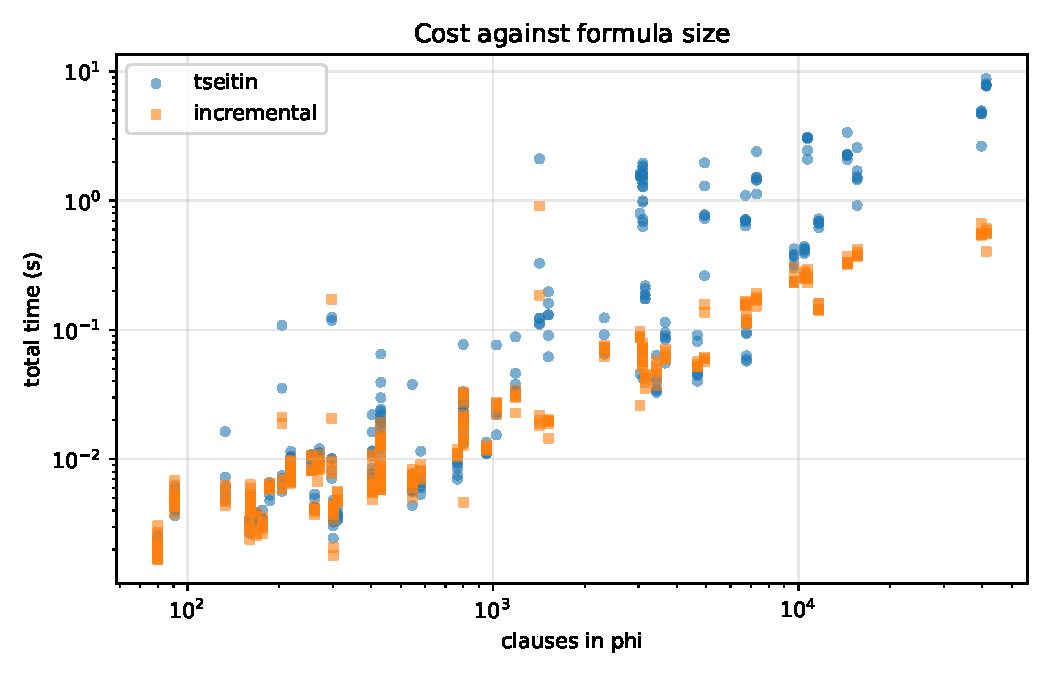
\includegraphics[width=0.72\textwidth]{figures/time_vs_size.pdf}
\caption{Total time of each run against the number of clauses of $\varphi$,
both axes logarithmic.}
\label{fig:time}
\end{figure}

Figure~\ref{fig:time} shows the same measurements per run rather than per
family. The two clouds overlap on the left, where the formulas are small, and
separate towards the right, with the Tseitin points rising faster. The spread
at a fixed size is wide for both approaches, which is the effect of instance
hardness noted above.

\begin{figure}[H]
\centering

\includegraphics[width=0.72\textwidth]{figures/calls_vs_size.pdf}
\caption{Number of solver calls against the number of clauses of $\varphi$,
both axes logarithmic.}
\label{fig:calls}
\end{figure}

Figure~\ref{fig:calls} makes the contrast between the two designs explicit.
The Tseitin approach is a flat line at two calls, one per direction, whatever
the size of the input. The incremental approach grows linearly with the number
of clauses, reaching $82\,415$ calls on the largest pair. Read together with
Figure~\ref{fig:time}, the two figures say that the number of calls is a poor
predictor of cost.

\begin{figure}[H]
\centering

\includegraphics[width=0.72\textwidth]{figures/phases.pdf}
\caption{Time spent building, loading and searching, summed over all runs.}
\label{fig:phases}
\end{figure}

Figure~\ref{fig:phases} shows the three phases side by side. Building and
loading are a visible part of the Tseitin bar and almost absent from the
incremental one, but the search dominates in both, so the cost of the Tseitin
approach is not merely the overhead of constructing a bigger formula. It is
that the formula it constructs is harder.

\subsection*{Early exit}

\begin{table}[H]
\centering
\begin{tabular}{lrrr}
\toprule
verdict & pairs & median calls & fraction of the maximum \\
\midrule
$\varphi \Leftrightarrow \psi$ & 345 & 860 & 100\% \\
$\varphi \Rightarrow \psi$ & 49 & 579 & 76\% \\
$\varphi \Leftarrow \psi$ & 35 & 987 & 100\% \\
none & 15 & 596 & 75\% \\
\bottomrule
\end{tabular}
\caption{Calls made by the incremental approach, by verdict. The maximum is
one call per clause in each of the two directions.}
\label{tab:early}
\end{table}

Table~\ref{tab:early} shows the effect of stopping at the first satisfiable
query. When the two formulas are equivalent every clause has to be checked in
both directions and the full number of calls is made. When an implication
fails, the direction that fails stops early, and the median run uses about
three quarters of the calls it would otherwise need. The saving is real but
modest here, because the failing direction is only half of the work and the
other half still has to run to completion.

\subsection*{Code}

All code is in \code{testing-equivalence/code/} and is available in the
repository~\cite{repo}.

\begin{itemize}
  \item \code{equivalence.py} holds the reader for DIMACS files, the two
  implication tests, and the function that combines two directional tests into
  a verdict. It also contains a reference implementation that enumerates all
  assignments, used only for the small correctness cases.

  \item \code{pairs.py} builds the second formula from the first by the six
  mutations, each recorded together with the verdict it is expected to give.

  \item \code{bench.py} runs the measurements and times the three phases. It
  reads \code{hardness.csv} to skip instances the solver cannot handle and
  applies the clause count limit described above.

  \item \code{probe.py} produces \code{hardness.csv} by attempting a plain SAT
  call on every instance in a child process with a hard cap, which is the only
  way to time out a single call.

  \item \code{test\_equivalence.py} contains the correctness checks: the small
  cases against enumeration, the verification of counterexamples, and the
  agreement of the two approaches.

  \item \code{experiments.ipynb} runs everything and writes \code{results.csv}
  and the figures used here.
\end{itemize}

\subsection*{Summary}

Both approaches were implemented and agreed on all $444$ pairs, which is the
main correctness result of the experiment.

On performance the outcome is one sided and contrary to what the number of
calls suggests. Making one call per clause of $\psi$ was $6.8$ times faster
overall than the single call on the Tseitin encoding, despite issuing about
three thousand times as many calls. The two approaches are equivalent on small
inputs and the gap grows with the size of the formula, reaching a factor of
ten on the largest family tested.

The explanation is that the two approaches do not give the solver the same
problem. The incremental approach always works on $\varphi$, which is loaded
once and never changes, and each query only adds a few assumptions that
usually conflict at once, so the learned clauses stay valid across all calls.
The Tseitin approach builds a new formula for every pair, larger than
$\varphi$ by one variable per clause of $\psi$, and that formula is harder to
solve than the one it came from. Its cost is dominated by search rather than
by construction, as Figure~\ref{fig:phases} shows.

The same asymmetry appeared while running the experiment. The Tseitin approach
is a single call and cannot be interrupted from inside the process, so one
instance with $233\,965$ clauses ran for twenty hours before it was stopped,
while the incremental approach is a loop and can give up between two calls.
That is a practical argument for the second approach beyond its speed.

\clearpage

\begin{thebibliography}{9}

\bibitem{satlib}
H. Hoos, T. St\"utzle, \emph{SATLIB: An Online Resource for Research on SAT}.
\url{https://www.cs.ubc.ca/~hoos/SATLIB/benchm.html}

\bibitem{pysat}
A. Ignatiev, A. Morgado, J. Marques-Silva,
\emph{PySAT: A Python Toolkit for Prototyping with SAT Oracles}, SAT 2018.
\url{https://pysathq.github.io}

\bibitem{cadical}
A. Biere, \emph{CaDiCaL}.
\url{http://fmv.jku.at/cadical}

\bibitem{repo}
Z. Ahmetovic, source code for this task.
\url{https://github.com/inferno73/SAT-solver-NAIL094}

\end{thebibliography}

\end{document}
